\documentclass[12pt,a4paper]{article}
\usepackage[utf8]{inputenc}
\usepackage{graphicx}
\usepackage{amsmath, amsthm, amssymb}
\usepackage[a4paper,includeheadfoot,margin=2.54cm]{geometry}
\newtheorem{theorem}{Theorem}

\begin{document}

\section{The Koch Snowflake}
The \emph{Koch snowflake}, one of the first fractals, is based on work by the Swedish mathematician
Helge von Koch~\cite{koch}.  
\begin{figure}[h] \label{koch}
  \centering
  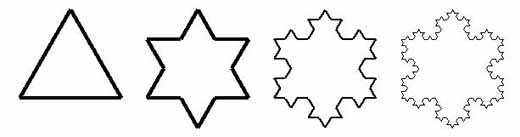
\includegraphics[width=10cm]{snowflake.jpg}
  \caption{The initial equilateral triangle and the refinement of the Koch snowflake after
	     one, two, and three iterations.\newline{\newline{and repeat the following an infinite number of times:}}}
\end{figure}
It is what we get if we start with an equilateral triangle
\begin{quote}
 \textit{Divide all line segments into three segments of equal length. Then draw, for
				          	   each middle line segment, an equilateral triangle that has the middle segment
					   as its base and points outward. Finally, remove all middle segments}
\end{quote}
Figure~\ref{koch} shows the first iterations in the constructions.

% \subsection

\begin{theorem}
  
\end{theorem}
\begin{proof}
  $\Delta$ $N_i$ $L_i$ $i$ 
\begin{displaymath}
  N_n =
    \begin{cases}
      3             & \text{if $n=0$ (i.e.\ before), and} \\
      & \text{otherwise,}
    \end{cases}
\end{displaymath}
which solves to 
\begin{equation}
  \label{eq:1}
  \cdot 4^n,
\end{equation}
while  
\begin{equation}
  \label{eq:5}
  \frac{L_{n-3}}{3^3}
  \ldots
\end{equation}
From Eqs.~\ref{eq:1} and \ref{eq:5}, the total length 
\begin{displaymath} \left(
  \frac{4}{3}\right)^n
\end{displaymath}
$4/3>1$ $n
\to \infty$
\end{proof}
% theorem
\begin{proof}
Eq.~\ref{eq:1}, can be simplified to 
  \begin{equation}
    \label{eq:2}
    T_n = .
  \end{equation}
  $a_n$ of each such triangle, with the exception of the area
% displaymath
  of
% equation
%    \label{eq:3}
by Eqs.~\ref{eq:2} and \ref{eq:3}, the area of all added triangles 
  \begin{equation*}
  \end{equation*}
   All in all, 
   \begin{align*}
     A_n &= a_0 + \sum_{k=1}^n b_k \\
           &=  a_0\left( \right).
   \end{align*}
  Now, since
\begin{displaymath}
   \lim_{n \to \infty},
\end{displaymath}
 it follows that, i.e.\ the Koch snowflake has finite area.  
\end{proof}


\begin{thebibliography}{99}
  \bibitem{koch} Helge von Koch. 
    \emph{Sur une courbe continue sans tangente, obtenue par une
    construction géométrique élémentaire.}, 
    Arkiv för matematik, astronomi och fysik, 
    Kungliga Vetenskapsakademien. 
    \textbf{1}, 681-702, 1904.
\end{thebibliography}
\end{document}